\chapter{From Discrete Observables to Interference}

This chapter follows Leonard Susskind's fourth lecture in the quantum mechanics sequence and keeps its order and emphasis: review first, replacement second, technical detour third, then the return to probabilities, then a new system, then the question of compatibility, and finally the two-slit experiment. The lecture itself is Leonard Susskind's; these notes also preserve selected blackboard evidence, with curation support acknowledged to LazyingArt LLC and Video2Book. The governing idea is that the postulates of quantum mechanics do not change when the observable becomes continuous, but the mathematical objects that express those postulates do.

\section{Review: Discrete Observables, Probabilities, and Basis States}

Let us begin exactly where the lecture begins: with a measurable quantity that can take discrete values. Call those values \(n=1,2,3,\dots\). If the system is in some state \(|\psi\rangle\), then a measurement returns one of these values with probability \(P(n)\), and the first rule is simply
\begin{equation}
\sum_n P(n)=1.
\end{equation}
The second rule is that the basis vectors associated with the different values of the observable may be taken to form an orthonormal basis:
\begin{equation}
\langle m|n\rangle=\delta_{nm}.
\end{equation}
Here \(\delta_{nm}\) is the Kronecker delta, equal to \(1\) when \(m=n\) and \(0\) otherwise. Susskind pauses to note that one may think of it as depending only on the difference \(n-m\); it is really the vanishing or nonvanishing of that difference that matters.

Probabilities are governed by amplitudes. In the discrete case the amplitude for obtaining the value \(n\) is \(\langle n|\psi\rangle\), and the probability is the squared magnitude of that amplitude:
\begin{equation}
P(n)=|\langle n|\psi\rangle|^2.
\end{equation}
So already, before any continuum enters, we have the full pattern: a basis of states, an inner product, amplitudes, and the rule that probabilities are obtained by squaring amplitudes.

\begin{figure}
\centering

\includegraphics[width=0.62\textwidth]{lecture_04_figure_02.png}
\end{figure}

The blackboard here still has the character of a review. The normalization and orthonormality relations are written cleanly at the top, while the probability picture is only beginning below. That is faithful to the lecture's rhythm: the picture is secondary; the formal rules are being re-established first.

If we plot the probability as a function of the discrete variable \(n\), the values live only on the integers. The picture is therefore not a continuous curve but a collection of heights, and it is those heights that add up to \(1\).

\begin{figure}
\centering
\begin{tikzpicture}[x=1.25cm,y=1.1cm]
\draw[->] (0,0) -- (5.0,0) node[right] {$n$};
\draw[->] (0,0) -- (0,3.0) node[above] {$P(n)$};
\foreach \x/\h in {1/1.8,2/0.9,3/1.35,4/0.6}
{
  \draw (\x,0) -- (\x,\h);
  \fill (\x,\h) circle (0.05);
}
\node[below] at (1,0) {$1$};
\node[below] at (2,0) {$2$};
\node[below] at (3,0) {$3$};
\node[below] at (4,0) {$4$};
\node at (3.35,2.35) {$\sum_n P(n)=1$};
\end{tikzpicture}
\end{figure}

This review is not detachable background. It is the template for everything that follows. Once the observable becomes continuous, sums will be replaced by integrals and Kronecker deltas by Dirac deltas, but the structure of the argument remains the same.

\section{From Discrete Probabilities to Continuous Probability Density}

Now let the observable be the position of a particle on a line. The first change is conceptual rather than algebraic. It no longer makes sense to ask for the probability that the coordinate is exactly equal to one particular real number. A single point has measure zero, and the probability of one exact value is therefore zero.

What does make sense is the probability that the particle lies in an interval. Susskind temporarily continues to use the symbol \(p\) for probability density, but to keep it separate from the later use of \(p\) for momentum, we will write the density as \(P(x)\). The probability that the particle is found between \(x\) and \(x+\Delta x\) is
\begin{equation}
P\bigl(x\in[x,x+\Delta x]\bigr)=\int_x^{x+\Delta x} P(x')\,dx'.
\end{equation}
Accordingly, the normalization rule becomes
\begin{equation}
\int P(x)\,dx=1.
\end{equation}
This is the first replacement. In the discrete case the probabilities themselves add to \(1\); in the continuous case the area under the density curve adds to \(1\).

\begin{figure}
\centering

\includegraphics[width=0.68\textwidth]{lecture_04_figure_03.png}
\end{figure}

The surviving frame is strong evidence for the geometry of the argument. The lecture is not yet doing something sophisticated here. It is making a simple point carefully: for a continuous variable, the physically meaningful probability is associated with a small interval and therefore with a small area under the graph.

\begin{figure}
\centering
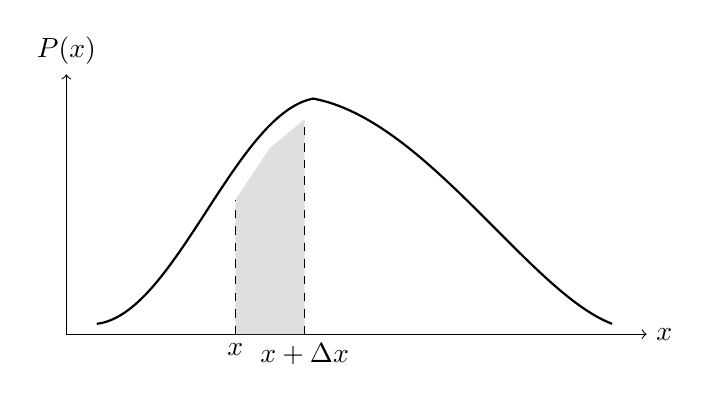
\begin{tikzpicture}[x=1.1cm,y=1.1cm]
\draw[->] (0,0) -- (6.7,0) node[right] {$x$};
\draw[->] (0,0) -- (0,3.0) node[above] {$P(x)$};
\draw[thick]
  (0.35,0.12)
  .. controls (1.25,0.22) and (1.95,2.55) ..
  (2.85,2.72)
  .. controls (4.15,2.48) and (5.35,0.48) ..
  (6.3,0.12);
\fill[gray!25]
  (1.95,0) --
  (1.95,1.55) --
  (2.35,2.15) --
  (2.75,2.48) --
  (2.75,0) -- cycle;
\draw[dashed] (1.95,0) -- (1.95,1.55);
\draw[dashed] (2.75,0) -- (2.75,2.48);
\node[below] at (1.95,0) {$x$};
\node[below] at (2.75,0) {$x+\Delta x$};
\end{tikzpicture}
\end{figure}

At this stage one replacement has been made: discrete probabilities have become probability densities. But a second replacement is now forced on us. If the basis is labeled by a continuous variable, what replaces \(\langle m|n\rangle=\delta_{nm}\)? Before returning to probabilities, the lecture deliberately steps aside to introduce the Dirac delta.

\section{The Dirac Delta and the Particle on a Line}

The Dirac delta is introduced as the continuous analogue of the Kronecker delta. Susskind presents it first in the intuitive way and only then in the operational one. Intuitively, \(\delta(x-y)\) is zero whenever \(x\neq y\), but at \(x=y\) it is concentrated into an infinitely narrow, infinitely tall spike of unit area:
\begin{equation}
\delta(x-y)=0 \quad \text{for } x\neq y,
\qquad
\int \delta(x-y)\,dx=1.
\end{equation}
As he says, no honest ordinary function behaves this way. But the spike picture is a good guide to how the object works.

The more careful statement is that the delta is defined by what it does under integration:
\begin{equation}
\int \delta(x-y)f(x)\,dx=f(y).
\end{equation}
Only the value of the function at \(x=y\) survives. The heuristic picture and the operational definition are not rivals here. In the lecture they play different roles. The spike picture carries the intuition; the integral rule carries the mathematics.

With that in hand, we can now write the continuum analogue of orthogonality:
\begin{equation}
\langle x|y\rangle=\delta(x-y).
\end{equation}
This is the natural replacement of \(\langle m|n\rangle=\delta_{nm}\) when the basis is labeled by position. If \(x\neq y\), the two position states are orthogonal; if \(x=y\), the overlap is concentrated at one point, exactly as the delta function prescribes.

\subsection{Question \& Answer}

\paragraph{Question.} How can \(\langle x|y\rangle\) be a delta function, and in what sense can a position eigenvector have infinite norm?

\paragraph{Answer.} The lecture answers this by not pretending the continuum is innocent. Instead, it backs up to a dense discrete approximation. Imagine replacing the line by a set of lattice sites separated by a tiny spacing \(a\), and let \(|n\rangle\) be the corresponding orthonormal basis:
\[
\langle n|m\rangle=\delta_{nm}.
\]
Now define the continuum-normalized position state by stretching the discrete state:
\[
|x\rangle=\frac{1}{\sqrt a}\,|n\rangle.
\]
If \(x\) corresponds to site \(n\) and \(y\) to site \(m\), then
\begin{equation}
\langle x|y\rangle=\frac{1}{a}\,\delta_{nm}.
\end{equation}
This object is zero unless the two sites coincide. When they do coincide, its height is \(1/a\). As \(a\) becomes very small, we get exactly the picture of a spike of width \(a\) and height \(1/a\), that is, the Dirac delta.

So yes, the continuum-normalized position states have divergent norm. But that is not a defect; it is the normalization convention adapted to continuum integration. One almost never needs \(\langle x|x\rangle\) by itself. What one actually uses is the delta function inside integrals, where it behaves perfectly well. The lecture's point is that the Dirac delta is not mysterious once one sees it as the rescaled limit of the Kronecker delta.

\section{Born's Rule in the Continuum}

Having inserted the delta-function detour, the lecture now returns, very explicitly, to the rules of probability. This return matters. Susskind is not content merely to quote \(P(y)=|\psi(y)|^2\). He wants to derive it from the same postulates used in the discrete case.

The states are now wavefunctions, that is, complex functions of a real variable \(x\), and the inner product on this vector space is
\begin{equation}
\langle \phi|\psi\rangle=\int \phi^*(x)\psi(x)\,dx.
\end{equation}
A particle known to be localized at the point \(y\) is represented in the \(x\)-representation by the wavefunction \(\delta(x-y)\). Therefore the amplitude to detect the particle at \(y\) in the state \(|\psi\rangle\) is
\begin{align}
\langle y|\psi\rangle
 &= \int \delta(x-y)\psi(x)\,dx \\
 &= \psi(y).
\end{align}
This is the formal version of a statement that is often introduced heuristically: the wavefunction evaluated at \(y\) is the amplitude to find the particle at \(y\).

Now we simply apply the probability postulate in its continuum form:
\begin{equation}
P(y)=|\langle y|\psi\rangle|^2.
\end{equation}
Using the previous result,
\begin{equation}
P(y)=|\psi(y)|^2=\psi^*(y)\psi(y).
\end{equation}
Susskind remarks that one could have begun with this formula directly. But the point of the lecture is different. The point is to show that nothing new has been added. We have simply taken the discrete postulates, replaced sums by integrals and Kronecker deltas by Dirac deltas, and then carried the same formal logic through.

The wavefunction of a particle on a line is therefore a probability amplitude in precisely the same sense that \(\langle n|\psi\rangle\) is a probability amplitude in the discrete case. The difference is only that the label on the basis is now continuous.

\section{Particle on a Circle: Periodicity, Momentum Eigenfunctions, and Quantization}

The next transition in the lecture is from one system to another, not from one formalism to another. We now study a particle moving on a circle of radius \(R\). To connect it with the line notation, the circle is cut and laid out as the interval
\[
0\le x\le 2\pi R.
\]
Everything looks the same as for a particle on a line until one remembers that this interval really came from a circle. That memory is encoded in one extra condition:
\begin{equation}
\psi(x+2\pi R)=\psi(x).
\end{equation}
The allowed state space is therefore the vector space of periodic complex functions on the interval. The lecture stops to note that this is indeed a vector space: multiplying a periodic function by any complex number keeps it periodic, and the sum of two periodic functions is periodic as well.

Now Susskind returns to momentum. In the \(x\)-representation, the momentum operator acts as
\begin{equation}
\hat p=-i\hbar\,\frac{\partial}{\partial x}.
\end{equation}
The frame below is the strongest board witness for the eigenvalue equation itself; the operator line above is only partly visible in the frame, but the transcript settles its standard form.

\begin{figure}
\centering

\includegraphics[width=0.68\textwidth]{lecture_04_figure_04.png}
\end{figure}

The momentum eigenvalue equation is
\begin{equation}
-i\hbar\,\frac{\partial}{\partial x}\psi(x)=p\,\psi(x).
\end{equation}
Solving it is immediate:
\begin{align}
\frac{d\psi}{dx}&=\frac{ip}{\hbar}\,\psi,\\
\psi_p(x)&=C\,e^{ipx/\hbar}.
\end{align}
So the momentum eigenfunctions are plane waves. This is one of the first places where the wave language of quantum mechanics becomes literal.

The lecture then normalizes the eigenfunctions on the circle.

\begin{figure}
\centering

\includegraphics[width=0.54\textwidth]{lecture_04_figure_05.png}
\end{figure}

The board shows the integrand \(\psi^*\psi\) and the measure \(dx\); the equality to \(1\) comes from the transcript rather than the frame. The normalization condition is
\begin{equation}
\int_0^{2\pi R}\psi_p^*(x)\psi_p(x)\,dx=1.
\end{equation}
Since \(\psi_p(x)=C e^{ipx/\hbar}\), we have \(\psi_p^*\psi_p=|C|^2\). Therefore
\begin{equation}
1=|C|^2\int_0^{2\pi R}dx=2\pi R\,|C|^2.
\end{equation}
Hence
\begin{equation}
C=\frac{1}{\sqrt{2\pi R}}
\end{equation}
up to an irrelevant phase, and the normalized eigenfunction is
\begin{equation}
\psi_p(x)=\frac{1}{\sqrt{2\pi R}}\,e^{ipx/\hbar}.
\end{equation}

For different eigenvalues \(p\neq q\), the corresponding eigenfunctions are orthogonal. One can check this directly, but the lecture prefers to emphasize the general reason: eigenvectors of a Hermitian operator with different eigenvalues are orthogonal. Thus
\begin{equation}
\int_0^{2\pi R}\psi_p^*(x)\psi_q(x)\,dx=0
\qquad
(p\neq q).
\end{equation}

The next frame is less legible mathematically, but it is valuable because it preserves the board layout: the explicit plane-wave form on one side and the bra-ket representation on the other.

\begin{figure}
\centering

\includegraphics[width=0.75\textwidth]{lecture_04_figure_06.png}
\end{figure}

The exact bra-ket label in the screenshot is partly obscured, so the following is a cautious transcript-based reconstruction:
\begin{equation}
\langle x|p\rangle=\frac{1}{\sqrt{2\pi R}}\,e^{ipx/\hbar}.
\end{equation}
That is, a momentum eigenvector, when written in the position basis, is a normalized plane wave.

Now comes the crucial new step. Not every plane wave is allowed, because the state must be periodic. Imposing periodicity gives
\begin{equation}
e^{ip(x+2\pi R)/\hbar}=e^{ipx/\hbar}.
\end{equation}
Cancelling the common factor \(e^{ipx/\hbar}\), we obtain
\begin{equation}
e^{i2\pi Rp/\hbar}=1.
\end{equation}
This happens precisely when the exponent is an integer multiple of \(2\pi i\):
\begin{equation}
\frac{2\pi Rp}{\hbar}=2\pi n,
\qquad n\in\mathbb Z.
\end{equation}
Therefore the allowed momenta are
\begin{equation}
p_n=\frac{n\hbar}{R}.
\end{equation}
The position on the circle is continuous, but the momentum is discrete. The lecture insists on the origin of this discreteness: it comes from periodicity of the wavefunction.

Now let \(L\) be the angular momentum. Classically,
\begin{equation}
L=Rp.
\end{equation}
Substituting the allowed momenta, we find
\begin{equation}
L_n=Rp_n=n\hbar.
\end{equation}
The factor of \(R\) disappears. Angular momentum is quantized in units of \(\hbar\), independent of the size of the circle.

\subsection{Question \& Answer}

\paragraph{Question.} Does the large-\(R\) limit give us classical mechanics, or only a dense momentum spectrum?

\paragraph{Answer.} Only a dense spectrum. As \(R\to\infty\), the spacing
\[
\Delta p=\frac{\hbar}{R}
\]
between neighboring momentum values goes to zero. The discrete spectrum becomes dense, and the lecture says that it is then convenient to pass from Kronecker-delta normalization to Dirac-delta normalization in momentum space. But nothing essentially classical has happened yet.

Classical mechanics would require that a particle could have a sharply defined position and a sharply defined momentum simultaneously. The large-\(R\) limit does not provide that. It merely makes the momentum eigenvalues closely packed. The real obstruction lies in the incompatibility of the position and momentum operators, which is the next topic.

\section{Compatibility, Common Eigenvectors, and the Commutator \([x,p]\)}

The lecture now answers the classical-limit question by shifting from eigenvalues to states. A dense spectrum is not enough. The issue is whether the system can be in a state that is simultaneously an eigenstate of position and momentum.

Suppose two observables are represented by operators \(A\) and \(B\). They are compatible if there exists a complete basis of vectors that are eigenvectors of both at once. Write
\begin{equation}
A|n\rangle=\alpha_n|n\rangle,
\qquad
B|n\rangle=\beta_n|n\rangle.
\end{equation}
Then
\begin{equation}
AB|n\rangle=\alpha_n\beta_n|n\rangle,
\qquad
BA|n\rangle=\beta_n\alpha_n|n\rangle.
\end{equation}
Since ordinary numbers commute, these two results agree. This leads to the criterion
\begin{equation}
[A,B]\equiv AB-BA=0.
\end{equation}
The lecture states, without proving it, that this is both necessary and sufficient: two observables are compatible precisely when their commutator vanishes.

Position and momentum do not satisfy this condition. Position eigenstates are sharply localized; momentum eigenstates are plane waves. On the circle, each momentum eigenstate has constant magnitude around the entire circle; on the infinite line, it is delocalized over the whole axis. So the lecture's physical point is immediate even before the algebra: these are not the same kind of states, and there are no common eigenvectors.

The algebra confirms this. Let \(x\) act by multiplication and \(p\) act as \(-i\hbar\,d/dx\). To determine the commutator, apply it to an arbitrary wavefunction \(\psi(x)\):
\begin{align}
(xp-px)\psi(x)
  &= x\left(-i\hbar\frac{d\psi}{dx}\right)
   -\left(-i\hbar\frac{d}{dx}\right)\bigl(x\psi(x)\bigr) \\
  &= -i\hbar\,x\frac{d\psi}{dx}
   + i\hbar\,\frac{d}{dx}\bigl(x\psi(x)\bigr).
\end{align}
Now use the product rule,
\begin{equation}
\frac{d}{dx}\bigl(x\psi(x)\bigr)=\psi(x)+x\frac{d\psi}{dx},
\end{equation}
so that
\begin{align}
(xp-px)\psi(x)
  &= -i\hbar\,x\frac{d\psi}{dx}
   + i\hbar\left(\psi(x)+x\frac{d\psi}{dx}\right) \\
  &= i\hbar\,\psi(x).
\end{align}
Because this is true for every \(\psi(x)\), we conclude that
\begin{equation}
[x,p]=xp-px=i\hbar.
\end{equation}

This is the formal hinge of the lecture. As a statement about ordinary numbers it would be nonsense, because \(xp=px\). But as a statement about operators it is exact. Susskind emphasizes that the right-hand side is just a number, and that is about as strong a failure of commutativity as one could have. There are no common eigenvectors at all.

The lecture also addresses a natural confusion here. Multiplication by \(x\) does not turn an arbitrary function into a constant multiple of itself. That is why generic functions are not eigenfunctions of the position operator. Only delta functions have the property that multiplication by \(x\) picks out one specific numerical value.

\section{Two-Slit Interference as Superposition of States}

The lecture now cashes out all of this formalism in the two-slit experiment. The central idea is not diffraction theory in detail. It is superposition. Quantum states can be added, and the probability is computed only after the amplitudes have been added.

Start with one hole open. The wave emerging from that hole spreads out and reaches the screen with a varying phase. Over a small region of the screen one may approximate the vertical dependence by something like \(e^{ipy}\), but Susskind is careful not to pretend that this is globally exact. A better heuristic description is
\begin{equation}
\psi_{\text{1-hole}}(y)\sim e^{i\varphi(y)}\rho(y),
\end{equation}
where \(\rho(y)\) is a slowly varying envelope and \(\varphi(y)\) is a rapidly varying phase. The lecture also gives a more geometric outgoing-wave model:
\begin{equation}
\psi(r)\sim \frac{e^{ipr}}{r},
\qquad
r=\sqrt{\ell^2+y^2}.
\end{equation}
The point of this formula is not to launch a full diffraction calculation. It is to explain why the local vertical frequency varies with \(y\). The phase is \(pr\), not simply \(py\), so as one moves away from the center the apparent oscillation in the vertical direction speeds up. In physical language, the particle must have picked up more vertical momentum.

\subsection{Question \& Answer}

\paragraph{Question.} Why does one hole give a smooth blob, while two holes can create dark fringes where no particle ever lands?

\paragraph{Answer.} For one hole, the phase may oscillate rapidly, but the probability is computed by multiplying the amplitude by its complex conjugate:
\begin{equation}
|\psi_{\text{1-hole}}(y)|^2
 \sim
 \bigl(e^{i\varphi(y)}\rho(y)\bigr)
 \bigl(e^{-i\varphi(y)}\rho(y)\bigr)
 = \rho(y)^2.
\end{equation}
The oscillating phase cancels. What remains is the smooth envelope. That is why a single hole can produce a broad blob even though the amplitude itself carries rapid phase variation.

With two holes open, however, the total state is the sum of two amplitudes:
\[
\psi=\psi_1+\psi_2.
\]
When we square that sum, cross-terms survive. Those cross-terms contain the relative phase, and that relative phase produces the interference pattern. So one hole gives a smooth probability because its phase disappears in \(|\psi|^2\); two holes give fringes because the relative phase does not disappear in \(|\psi_1+\psi_2|^2\).

To see the algebra in the form used in the lecture, let us work locally on the screen and choose units in which \(\hbar=1\). Approximate the two contributions by
\begin{equation}
\psi_1(y)\approx e^{ipy},
\qquad
\psi_2(y)\approx e^{iqy}.
\end{equation}
Each one separately has constant magnitude. Hence each one separately would give a uniform probability over that small interval. But with both holes open,
\begin{align}
|\psi_1+\psi_2|^2
 &= (e^{ipy}+e^{iqy})(e^{-ipy}+e^{-iqy}) \\
 &= 1+1+e^{i(p-q)y}+e^{i(q-p)y} \\
 &= 2+2\cos\bigl((p-q)y\bigr).
\end{align}
This is not constant. It oscillates, and for those values of \(y\) where the cosine is \(-1\), the probability is zero. These are the dark fringes.

That is the lecture's real payoff. Open one hole and a particle can arrive at a given point. Open the other hole and it can arrive there as well. Open both holes together and there are points that no particle reaches in the idealized limit. This is not because probabilities were added incorrectly; it is because amplitudes were added first, and only then squared.

The lecture repeatedly returns to the particle character of the phenomenon. One sends particles through one at a time. Each event is just a spot on the screen. But after many repetitions the spots build up the probability distribution. The distribution is always nonnegative, because it comes from an amplitude times its complex conjugate, but it need not be strictly positive. In the ideal limit it can vanish.

The dependence on slit separation now reads like ordinary beats. If the two holes are very close together, the local vertical frequencies \(p\) and \(q\) are almost the same, so \(p-q\) is small and the cosine varies slowly. The fringe spacing is therefore large. If the holes are farther apart, \(p-q\) is larger and the fringes become more closely spaced.

The lecture also adds a useful caution. A single aperture with sharp edges can itself produce diffraction structure because each edge behaves as a secondary source. That is a different effect. The point here is the distinct and stronger interference that arises from the superposition of the states associated with two separate holes.

Finally, the lecture stops at exactly the right place. It refuses, for the time being, to answer the which-path detector question. If a detector tells us which slit the particle went through, the interference pattern is destroyed, but to explain that properly one needs composite systems and entanglement. The same is true of the reversibility question that comes up at the end. Those topics are deferred until Hamiltonians, evolution, and tensor-product structure are in place.

\section{Summary}

The lecture unfolds as one deliberate chain of replacements and payoffs. We begin with the discrete case: probabilities \(P(n)\), orthonormal basis states, amplitudes, and the Kronecker delta. We then pass to continuous variables: exact point-probabilities give way to interval probabilities, sums become integrals, and the Kronecker delta becomes the Dirac delta. With those replacements in hand, the continuum Born rule follows from the same abstract postulates:
\[
P(y)=\psi^*(y)\psi(y).
\]
The move from the line to the circle changes not the formalism but the allowed state space, and periodicity then forces momentum and angular momentum to be quantized. The student's natural question about the large-\(R\) limit pushes the lecture to the deeper issue of compatibility, culminating in the operator identity
\[
[x,p]=i\hbar.
\]
That identity explains why position and momentum are not simultaneously sharp. The two-slit experiment then gives the physical payoff: amplitudes add, probabilities do not, and the cross-term in
\[
|\psi_1+\psi_2|^2
\]
creates an interference pattern with genuine dark fringes. The lecture ends by leaving the detector question open, not because it is unimportant, but because it belongs to the next layer of the subject.